\chapter{Teoretická část}\label{chapter:resere}
Tato kapitola obsahuje základní teoretickou informaci o~technologiích, které jsou použity v~současné implementaci aplikace a také o~technologiích, které budou použity při implementaci a analýze.

\section{Pravidla frameworku Angular pro Git}\label{reserse:git}
    V~této bakalářské práci nebude použit framework Angular. Prozkoumaná pravidla nebyla kompletně převzata, ale byla provedena analýza a následně byly převzaté části pravidel, které jsou použitelné při implementaci serveru, který je předmětem této bakalářské práce. Kompletní přehled pravidel se nachází na GitHub\footnote{ GitHub je webová platforma pro vývoj softwaru pomocí systému řízení verzí Git.}\cite{angular-git}.
    
    Pravidla, která byla použita v~této bakalářské práci, definují formátování pro \verb|commit|\footnote{Proces, při kterém se uloží všechny provedené změny v~rámci systému řízení verzí a zařadí se do historie změn.} v~rámci verzovacího systému Git\footnote{je distribuovaný systém řízení verzí}. Příčinou zavedení konvencí je potřeba zpřehlednění grafu větví. Po dokončení této bakalářské práci, bude server kompletně funkční, ale proces vývoje tím neskončí. Budoucí kroky budou podrobně popsány v~kapitole \ref{zhodnocení}. Pochopení jednotlivých změn provedených během vývoje softwaru, pomáhají srozumitelné popisy jednotlivých změn. Dosažení takového výsledku pomáhá zavedení jednotného formátu pro každý \verb|commit| v~rámci projektu.
    
    \begin{figure}
            \begin{minted}{text}
<type>(<scope>): <subject>
<BLANK LINE>
<body>
<BLANK LINE>
<footer>
            \end{minted}
            \caption{Formát pro \texttt{commit} podle pravidel definovaných pro framework Angular} 
            \label{code:angular-commit}
    \end{figure}
    \begin{figure}
	   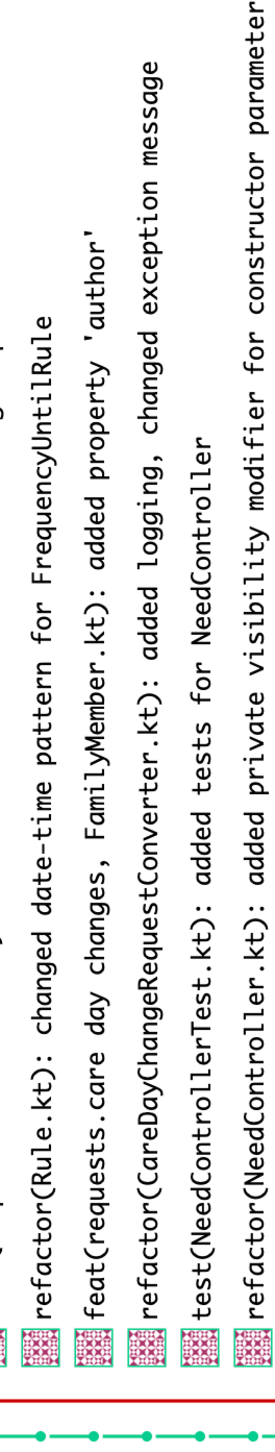
\includegraphics[angle=-90, width=1.0\textwidth]{pdfs/GitLabTree}
	   \caption[Ukázka použití konvence pro práci z~Git]{Ukázka použití konvenci pro práci z~Git na grafu větví}\label{image:gitlab-tree}
    \end{figure}
    Po provedení analýzy pravidel, pravidla byly opraveny podle potřeb tohoto projektu, ale struktura jednotlivé nebyla změněna. Konvence byla zavedena na začátku práce autora na implementaci této bakalářské práce a neměnila se během vývoje. Na obrázku \ref{image:gitlab-tree}) je zobrazen kus grafů větví GitLab po zavedení pravidel. V~následujících podsekcích bude uveden podrobný popis výsledných pravidel po úpravách autora. Struktura pro \verb|commit|, která je definovaná ve zdroji, se skládá ze pěti částí (viz obrázek \ref{code:angular-commit}):
    \begin{itemize}
    \setlength\itemsep{0.3em}
        \item \texttt{typ};
        \item \texttt{rozsah};
        \item \texttt{předmět};
        \item \texttt{tělo};
        \item \texttt{zápatí}.
    \end{itemize}
    
    \subsection{Typ}
        Typ definuje část aplikace, kterou provedený \verb|commit| mění. Seznám hodnot, které je možné zadat, je omezený předem definovaným seznamem:
        \begin{itemize}
        \setlength\itemsep{0.3em}
            \item \texttt{build} -- změny procesu sestavení aplikace nebo úpravy externích závislostí;
            \item \texttt{ci} -- změny týkající se průběžné integrace;
            \item \texttt{docs} -- změny týkající se jenom dokumentace;
            \item \texttt{feta} -- přidání nových funkcí;
            \item \texttt{fix} -- oprava chyb;
            \item \texttt{perf} -- změny zvyšující efektivitu;
            \item \texttt{refactor} -- změny, které nepřidávají nové funkce a současně neopravují chyby;
            \item \texttt{style} -- změny, které nemění význam kódu;
            \item \texttt{test} -- přidaní nebo úprava testů.
        \end{itemize}
    
    \subsection{Rozsah}
        Rozsah definuje konkrétní soubory nebo balíčky, které byly změněny. Uvedený rozsah není povinný, ale v~rámci této bakalářské práce bude rozsah uveden pro každý \verb|commit|. V~případě, že změny byly provedeny současně v~několika různých souborech nebo balíčcích, je potřeba uvést je jako seznam s~položkami v~kulatých závorkách oddělenými čárkami.
    
    \subsection{Předmět}
        Předmět je stručným popisem provedených změn. Změny mají být odděleny od typu dvojtečkou. V~případě, že \verb|commit| obsahuje několik změn, je potřeba je oddělit čárkou. První písmeno každé změny musí být malé. Poslední změna nekončí tečkou.
    
    \subsection{Tělo}
        Tělo je určeno pro podrobnější popis provedených změn. Tato část není povinná, ale je doporučena v~případě, že provedené změny nejsou pochopitelné po přečtení předmětu nebo není jasná příčina provedené změny.
    
    \subsection{Zápatí}
        Zápatí je určeno pro definování přelomových změn a definování závislostí na konkrétní požadavky v~rámci GitHub nebo GitLab\footnote{Webová platforma pro vývoj softwaru pomocí systému řízení verzí Git.}. V~rámci této bakalářské práce jsou každému požadavku v~rámci GitLab přiděleny jednotlivé větve, proto není potřeba uvádět identifikátor požadavku v~zápatí.
    
\section{Použitý jazyk programování}\label{resere:kotlin}
    Současný návrh aplikace byl proveden v~jazyce Kotlin, který je relativně novým jazykem pro JVM\footnote{Java Virtual Machine.}. Poprvé byl tento jazyk představen společností JetBrains v~roku 2011. V~této bakalářské práci byla použita verze 1.3.72 . V~porovnání s~Javou, jejíž podpora je dlouhodobě zaručena společností Oracle, nemá Kotlin předem definovanou periodu podpory, ale podle oficiálních webových stránek zaručuje zpětnou kompatibilitu pro alespoň jednu stabilní verzi, což dovoluje pohodlně migrovat do novější verze jazyka.\cite{java-support-period}\cite{kotlin-compatibility}
    
    %===================================================================
    % Kotlin je relativně nový jazyk pro JVM\footnote{Java Virtual Machine}. Poprvé tento jazyk byl představen společnosti v 2011 roku. První stabilní verze byla představena v únoru roku 2016. Ale už v květnu roku 2017 Kotlin se stal oficiálním jazykem pro Android.
    
    % https://kotlinlang.org/docs/reference/
    Kotlin byl vytvořen jako alternativa k~jazyku Java a řeší některé jeho problémy. Například, Kotlin řeší problém použití \texttt{null}, také známý jako \texttt{The Billion Dollar Mistake}, a problémy s~ním spojené. Java samotna nemá podporu pro \texttt{not-null} proměnné, ale Kotlin takovou podporu má nativně, a to v~podobě oddělení \texttt{nullable} typu pomocí ? operátoru. Pro kompletní seznámení s~jazykem Kotlin je doporučeno navštívit oficiální webové stránky, kde najdeme podrobný návod k~použití jazyka.\cite{kotlin-documentation}
    

\section{Nástroj pro automatizaci sestavování programu}\label{resere:build}
    % https://gradle.org/maven-vs-gradle/
    % https://www.baeldung.com/ant-maven-gradle
    Pro automatizaci sestavování programu se používá nástroj Gradle, který už se používá v~současné implementaci aplikace. Existuje populární alternativa -- Maven, ale Gradle je modernější a pohodlnější. Konfigurace se provádí v~jazyce Groove nebo přímo v~jazyce Kotlin. Také Gradle poskytuje možnost definovat vlastní úkoly spustitelné pomocí příkazové řádky, které pak budou využité pro analýzu a spuštění testů. Podrobnější informaci o~porovnání nástrojů Gradle a Maven lze najít na stránkách \cite{grale-vs-mavem} a \cite{gradle-vs-maven-bealdung}.

\section{Nástroj pro vývoj podnikových aplikací}\label{resere:j2ee}
    % https://spring.io/projects/spring-framework
    % https://spring.io/projects
    % \cite{spring-framework}
    Spring je jeden z~nejznámějších frameworků určených pro vývoj podnikových aplikací. Infrastruktura Spring je velká a komplikovaná. V~době práce na této bakalářské práci se Spring skládal ze 24 aktivních projektů. V~rámci této bakalářské práce bude využito současně několik různých projektů, které zajišťují korektní funkčnost různých aspektů serveru. V~této sekci budou popsány jenom projekty, které budou následně využity při implementaci. Popis je velice stručný a je uveden za účelem pochopení základů použitých technologií. Pro podrobnější informace o~zmíněných projektech je doporučeno navštívit oficiální webovou stránku \cite{spring-projects}.
    
    \subsection{Spring framework}
        Spring framework je základem pro ekosystém různých projektů, které budou popsány v~následujících sekcích.\cite{spring-framework} Tento nástroj samotný je správcem závislostí (\textit{dependency manager}). Spravování závislostí je reprezentováno pomocí principu \texttt{Inversion of Control} (IoC), což znamená, že framework Spring je kontejnerem, který je zodpovědný za vytváření objektů a jejich provázáním mezi sebou. Konfigurace aplikace je reprezentována pomocí rozhraní \texttt{ApplicationContext}.
        
        \begin{figure}
            \begin{minted}{yaml}
spring.profiles.active=dev
            \end{minted}
            \caption{Příklad definování profilu aplikace pomocí proměnné prostředí} 
            \label{code:current-spring-profile}
        \end{figure}
        Pro pohodlnou práci a zvýšení efektivity napsaného kódu má Spring množství dalších užitečných řešení. Jak už bylo zmíněno, popisovat všechno nemá smysl, ale několik nejdůležitějších věcí není možné opomenout. První funkce, která bude široce využita při implementaci, se týká proměnných v~rámci prostředí aplikace. Tyto proměnné umožňují definovat důležité proměnné pro konfiguraci běhu aplikace zvlášť od jejich využití v~kódu. Framework Spring umožňuje využít tyto proměnné přímo v~kódu. Implicitním souborem obsahujícím tyto proměnné je soubor \texttt{application.properties}. Pro zavedení různých proměnných pro různé případy použití aplikace je možné definovat několik takových souborů pro každý z~profilů. Jedinou věcí, kterou je potřeba udělat, je vytvořit soubor, který bude mít v~názvu jméno profilu, kterému patří (\texttt{application-{profile}.properties}). Pro definování, který profil má aplikace použit v~následujících spouštěních, je potřeba v~implicitním souboru zadat potřebný profil jako proměnnou (viz obrázek \ref{code:current-spring-profile}). 
        
        
        \begin{figure}
            \begin{minted}{Kotlin}
@Bean
@ConditionalOnProperty(
        value = ["scheduled.alimonyFactory"],
        matchIfMissing = false,
        havingValue = "true")
fun startAlimonyFactory(): AlimonyFactory {
    logger.info("Schedule job: starting AlimonyFactory")
    return AlimonyFactory(
            alimonySettingRepository,
            alimonyRepository)
}
            \end{minted}
            \caption{Příklad aspektově orientovaného programování v~Spring} 
            \label{code:spring-conditional}
        \end{figure}
        Spring framework používá techniku vkládání závislosti (\textit{dependency injection}), což dává možnost psaní kvalitnějšího softwaru, ale Spring poskytuje možnost zlepšit výsledný kód ještě více. Framework Spring také používá paradigma aspektově orientovaného programování (AOP). Toto paradigma má za cíl zvýšit modularitu výsledného softwaru pomocí rozdělení kódu do logických částí, nalezení opakujících se částí, které jsou také nazývané průřezové problémy, a nahrazení opakujícího se kódu. Příkladem AOP je anotace zaměřená na podmíněné spouštění metody v~závislosti na výsledku předem definované podmínce v~závorkách (viz obrázek \ref{code:spring-conditional}).
    
    \subsection{Spring Boot}
        % https://docs.spring.io/spring-boot/docs/current/reference/html/spring-boot-features.html#boot-features-external-config
        Spring Boot je pomocný nástroj pro programátora při konfiguraci aplikace využívající framework Spring. Spring Boot registruje 17 různých implicitních zdrojů proměnných. Kompletní popis zdrojů je na oficiálních stránkách dokumentace \cite{spring-property-sources}. Podle nalezených proměnných framework provádí analýzu konfigurace aplikace a následně, pomocí anotací pro podmínky, automaticky nastavuje prostředí aplikace. Navíc od klasického frameworku Spring, Sping Boot obsahuje rozšířený seznam anotací pro podmínky, které jsou široce využity pro zmíněnou automatickou konfiguraci.\cite{spring-boot}
    
    \subsection{Spring Security}
        Spring Security je framework určený pro návrh autentizace, autorizace a filtrů. Framework vyžaduje využití frameworku Spring, případně i frameworku Spring Boot. Podrobné informace lze najít na oficiálních stránkách \cite{spring-security}.
    
    \subsection{Spring Data}
        % https://docs.spring.io/spring-data/jpa/docs/current/reference/html/#repositories.query-methods
        Spring Data je framework pro pohodlnou práci programátora při implementaci datové vrstvy\footnote{Vrstva aplikace, která komunikuje s~databází.}. Framewok vytváří dodatečnou vrstvu nad implementací Java Persistense API\footnote{Application programming interface.} (JPA). Implementací JPA může být EclipseLink nebo Hibernate. Příkladem využití je rozhraní \texttt{CrudRepository}, které bude využito v~této bakalářské práci. Rozhraní definuje základní operace s~databází a dovoluje programátorovi jenom definovat typ entity a typ primárního klíče. V~případě, že programátor potřebuje složitější dotazy na databázi, framework poskytuje možnost definování metod, které ve svých názvech obsahují popis dotazů~\cite{query-methods}. Framework rozebírá název na jednotlivé části a překládá ho na SQL\footnote{Structured Query Language.} dotaz.
    
    \subsection{Spring Web Services}
        Spring Web Services je framework určený pro implementaci webových služeb. V~rámci této bakalářské práce bude tento framework využit pro implementaci aplikační vrstvy serveru. Aplikační vrstva aplikace má pokrývat případy užití aplikace. Podrobnou informaci lze najít na oficiálních stránkách~\cite{spring-web-services}.
        

%  \section{Spring Boot}\label{reserse:spring-boot}
    % https://spring.io/projects/spring-boot
    % \cite{spring-boot}
    % TODO Spring Boot je nástrojem určeným pro rychlý a
    
\section{Testování}\label{reserse:testovani}
    Testování aplikace se skládá z~několika částí. První část je testování softwaru samotného pro ověření jestli jednotlivé metody, třídy nebo celé moduly fungují správně a komunikují mezi sebou bezchybně. Druhou částí testování je ověření, jestli testy pokrývají dostatečnou část kódu a jestli pokrývají důležité funkce. V~této sekci jsou popsány nástroje pro zaručení kvalitního testování, které budou následně využity při implementaci testů a jejich analýze.
    
    \subsection{Spring}
        Framework Spring poskytuje velký počet nástrojů pro testování softwaru. Každý z~dodatečných frameworků, jako Spring Boot nebo Spring Security, spolu s~novými funkcemi, přidávají vhodné nástroje pro kvalitní testování těchto funkcí. Celý přehled nástrojů, které poskytuje framework, je na oficiálních stránkách dokumentace~\cite{spring-tests-doc}. V~této sekci jsou uvedeny jenom nejdůležitější použité nástroje.
        
        Prvním nástrojem je anotace \texttt{SpringBootTest}, kterou poskytuje framework Spring Boot pro implementaci integračních testů. Při použití této anotace framework vytvoří nutný kontext aplikace pro kompletní testování.
        
        Druhým důležitým nástrojem je třída \texttt{MockMvc}, která poskytuje možnost kvalitního testování aplikační vrstvy serveru. Tento nástroj je součástí frameworku Spring Web Services.
        
    \subsection{JUnit}
        JUnit je framework určený pro testování softwaru. V~této bakalářské práci bude použita verze 5. Tento framework bude použit pro vytvoření kostry testování. Podrobnější informace o~funkcích frameworku je dostupná na oficiálních webových stránkách~\cite{junit-doc}.
        
    \subsection{JaCoCo}\label{resere:testovani:jacoco}
         %https://www.jacoco.org/jacoco/trunk/doc/implementation.html
        JaCoCo je nástroj poskytující podrobnou analýzu testů. Tento nástroj bude použit pro výslednou analýzu implementovaných testů a také jako pomocný nástroj pro nalezení důležitých neotestovaných funkcí během implementace testů. Nástroj existuje v~reprezentaci přídavného modulu pro nástroj Gradle, který se již používá v~současné implementace programu. Výsledky práce jsou následně uloženy do předem definované složky a jsou reprezentovány pomocí HTML\footnote{Hypertext Markup Language.} stránek. Nástroj je otevřeným softwarem, proto podrobnou informaci o~implementaci lze najít na oficiálních stránkách~\cite{jacoco-implementation}. Výsledky analýzy podle JaCoCo jsou dostupné v~příloze \ref{dodatek:code-coverage}.
        
    \subsection{IntelliJ IDEA}\label{resere:testovani:intellij-idea}
        % https://www.jetbrains.com/help/idea/code-coverage.html
        % TODO nastroj pro analyzu pokryti kodu testy \cite{intellij-idea-code-coverage}
        Pro provedení analýzy testů také bylo využito vývojové prostředí IntelliJ IDEA, používané autorem této práce pro implementaci programu. Nástroj pro pokrytí kódu testy je implicitním nástrojem zmíněného vývojového prostředí a poskytuje možnost zobrazování výsledků analýzy přímo v~kódu. Takový přístup zrychluje proces implementace testů. Nástroj také dovoluje vygenerovat výsledky zvlášť od kódu, proto tyto výsledky jsou také dostupné v~příloze \ref{dodatek:code-coverage}.


\section{Dokumentace}\label{resere:dokumentace}
    Pro dokumentace API v~současné implementaci aplikace se používá framework Swagger. Důležitou funkcí, kterou framework poskytuje, je automatické generování dokumentace na základě přidaných anotací v~kódu. Dokumentace je následně dostupná z~internetu ze stejné adresy jako server, ale na jiném portu. Podrobná informace o~framewoku je dostupná na oficiálních webových stránkách~\cite{swagger-doc}.
    
\section{Použité databáze}\label{resere:databaze}

    \subsection{H2}
        % Pro proces vývoje a testování byla zvolena databáze H2\cite{h2-db}, která je relační databází. 
        % http://www.h2database.com/html/tutorial.html
        Současná implementace používá relační databáze H2. Hlavním důvodem zvolení právě této databáze je možnost volby několika různých režimů, kde jeden z~režimu je vestavěný režim. Tento režim usnadňuje programátorovi práci s~databází, protože se databáze vytváří při spuštění programů a zaniká při jejich zastavení. Soubory s~daty jsou uloženy na disku nebo přímo v~paměti. H2 má též vlastního manažera, který je dostupný přes webový prohlížeč. Podrobnější informace jsou dostupné na oficiálních webových stránkách~\cite{h2-doc}.
        
    \subsection{PostgreSQL}
        % https://www.postgresql.org/docs/12/index.html
        % https://docs.spring.io/spring-cloud-dataflow/docs/1.1.0.RELEASE/reference/html/configuration-rdbms.html
        PostgreSQL je široce využívanou objektově relační databází napsanou v~jazyce C. V~době odevzdání této bakalářské práce je databáze PostgreSQL udržována skupinou Global Development Group a je otevřeným softwarem. Pro implementaci byla zvolena poslední stabilní verze -- 12. Kompletní dokumentace je dostupná online~\cite{postgres-documentation}. Framework Spring, zmíněný v~sekci \ref{resere:j2ee}, nativně podporuje použití PostgreSQL.
        

\section{Nástroj pro analýzu rozsahu implementace}\label{reserse:cloc}
    Nástroj CLOC\footnote{Count Lines of Code.}\cite{cloc-download} poskytuje možnost spočítat počet řádek kódu je v~dané složce. Nástroj podporuje velký počet programovacích jazyků programování. Výsledek obsahuje počet řádek kódu oddělený od komentářů a prázdných řádek. Tento nástroj bude použit pro analýzu současné implementace aplikace a analýzu provedené práce v~rámci bakalářské práce.